
%%%%%%%%%%%%%%%%%%%%%%%%%%%%%%%%%%%%%%%%%%%%%%%%%%%%%%%%%%%%%%
% NUbots' TDP 2014
%
% Date: 08.02.2014
%
%
\documentclass{llncs}
%
\usepackage{graphicx}
%
\begin{document}
%

\frontmatter          % for the preliminaries
%
\pagestyle{headings}  % switches on printing of running heads
\addtocmark{The NUbots Qualification material for RoboCup 2014} % additional mark in the TOC
%
%
\mainmatter              % start of the contributions
%
\title{The NUbots Team Description Paper 2014}
%
\titlerunning{The NUbots Team Description for 2014}  % abbreviated title (for running head)
%                                     also used for the TOC unless
%                                     \toctitle is used

\author{Brendan Annable \and David Budden \and Sophie Calland \and Stephan K. Chalup \and Shannon K. Fenn \and Madison Flannery \and Jake Fountain \and Robert A.R. King \and Alexandre Mendes \and Mitchell Metcalfe \and Steven P. Nicklin \and Peter Turner \and Josiah Walker}
%
\authorrunning{Annable et al.}   % abbreviated author list (for running head)
%
%%%% modified list of authors for the TOC (add the affiliations)
%\tocauthor{S.K. Chalup, A. Mendes, R.A.R. King, D. Budden, S. Fenn}
\tocauthor{B. Annable, D. Budden, S. Calland, S.K. Chalup, S. Fenn, M. Flannery, J. Fountain, R.A.R. King, A. Mendes, M. Metcalfe, S.P. Nicklin, P. Turner, J. Walker}
%
\institute{Newcastle Robotics Laboratory\\ School of Electrical Engineering \& Computer Science\\
Faculty of Engineering and Built Environment\\
The University of Newcastle, Callaghan 2308, Australia\\
Contact: \email{stephan.chalup@newcastle.edu.au}\\
Homepage: \texttt{http://robots.newcastle.edu.au}}
%

\maketitle              % typeset the title of the contribution

\begin{abstract}
The NUbots team, from The University of Newcastle, Australia, has had a strong record of success in the RoboCup Standard Platform League since first entering in 2002. The team was also competitive within the RoboCup Humanoid Kid-Size League since 2012. The 2014 team comprises several new students. This paper summarizes the history of the NUbots team, describes the roles and research of the team members, gives an overview of the NUbots' robots and software system, and addresses relevant research projects within the the Newcastle Robotics Laboratory.
\end{abstract}

%
\section{Introduction}
%
The NUbots team, from the University of Newcastle, Australia, competed in the Four Legged League from 2002-2007, within the Standard Platform League from 2008-2011 and subsequently within the Kid-Size Humanoid league since 2012. The NUbots have had a strong record of successes, twice achieving a first place; in 2006 in Bremen, Germany, and, again in 2008 as part of the NUManoid team in Suzhou, China.

The central goal of the NUbots is to be a high performance competitive robot soccer team at RoboCup. The vision of the research projects associated with the NUbots team is to develop and program robots that can support humans not only for routine, challenging, or dangerous tasks, but also to improve quality of life through personal assistance, companionship, and coaching.  Our mission is to contribute to a responsible development and application of robotics. Some of our projects therefore emphasize anthropocentric and biocybernetic
aspects in robotics research~\cite{ChalupOstwald2009}. This includes new aspects of human robot interaction and perception. The Newcastle Robotics Lab hosts several postgraduate and undergraduate research projects that are associated with the NUbots.

%The following sections describe the history of the team, the roles and research of the team members and addresses associated research projects and relevant aspects of the study and research environment of the University of Newcastle, Australia.

\section{Commitment to RoboCup 2014}
The Nubots commit to participation at RoboCup 2014 upon successful qualification. We also commit to provision of a person, with sufficient knowledge of the rules, available as referee during the competition.

\section{History of the NUbots' participation at RoboCup}
%The University of Newcastle's RoboCup initiative started in 2001. After the introduction of new robotics and machine learning
%related courses and projects two undergraduate students participated in RoboCup Junior in Seattle and won the world title.

The NUbots team was founded in 2002 and participated for the first time at RoboCup in Fukuoka in the Sony Four-Legged League (3rd place). Since then the team has  a strong history of competition and success in the RoboCup SPL/Four-Legged League, obtaining many top three placements and winning the title in 2006 and 2008.

During the previous two years the NUbots SPL code base has been ported to the DARwIn-OP platform and the majority of modules previously used on the NAO robot in the SPL were fielded for RoboCup 2012. Since then the majority of modules have undergone major revision in order to allow more effective use of the newer platform and in response to recent changes in the league rules. 

\section{Background of the NUbots Team Members}
\begin{itemize}
\item \emph{Josiah Walker} is studying for a Doctorate of Philosophy in Computer Science in Reinforcement Learning and Robotics. He works on robot behaviour and machine learning for various NUbot systems. He is the NUbots team leader for 2013.




\item \emph{Brendan Annable} is a 2nd year undergraduate student studying Software Engineering currently working on network infrastructure as well as a browser-based debugging environment.

\item \emph{Sophie Calland} is a third year undergraduate student studying Computer Engineering and Computer Science. She is working on the NUbots configuration system to consolidate system parameters.

\item \emph{A/Prof. Stephan Chalup} is the head of the Newcastle Robotics
Laboratory. He is an Associate Professor in Computer Science and Software Engineering.
He is one of the initiators of the University of Newcastle's
RoboCup activities since 2001. His research area is machine learning
and anthropocentric robotics.

\item \emph{Shannon Fenn} is in the final semester of a Computer Engineering and Computer Science degree, who completed his Honours thesis on shape-based computer vision and optimisation, his works on machine vision with a focus on geometric methods.

\item \emph{Madison Flannery} is a 3rd year Computer Science undergraduate currently working on improving the detection of field objects in the NUbots vision system.

\item \emph{Jake Fountain} is a fourth year undergraduate student studying a combined degree in mathematics and science, with his main interests lying in machine learning and artificial intelligence.

\item \emph{Dr. Robert King} is a Lecturer in Statistics at the University of Newcastle. His research focus is on flexibly-shaped distributions,
statistical computing and Bayesian knowledge updating. He joined the
NUbots in 2004 and has developed a special interest in RoboCup rules and refereeing.

\item \emph{Mitchell Metcalfe} is a fourth year undergraduate student studying combined degree in Mathematics and Computer Science. He is working on the NUBots' configuration system to consolidate system parameters.

\item \emph{Peter Turner} is technical staff in the School of Electrical Engineering and Computer Science. He is an expert on robot hardware and electronics and familiar with the Darwin-OP.
\end{itemize}

We also acknowledge the input of colleagues from the Newcastle Robotics Laboratory, team members of previous years
and the Interdisciplinary Machine Learning Research Group (IMLRG) in
Newcastle, Australia. Details are linked to the relevant webpages at
\texttt{www.robots.newcastle.edu.au}. Other robotics lab members who have contributed over the past six months include:
\begin{itemize}

\item \emph{David Budden} is a recent Computer Engineering and Computer Science graduate, who completed his Honours thesis on colour-based computer vision and bipedal robotic locomotion.

\item \emph{Dr. Alexandre Mendes} is deputy head of the Newcastle Robotics
Lab. He is a Senior Lecturer in Computer Science and Software Engineering.
He joined the group in September 2011 and his research areas are algorithms and optimisation.

\item \emph{Steven Nicklin} is studying for a Doctor of Philosophy in the robotics lab. He has been working on localisation and modelling of the robot. Steve has been NUbots team leader several times and was member of the world champion teams in 2006 and 2008.



\end{itemize}



%\pagebreak
\section{Hardware and Software Overview}
The NUbots use the DARWIN-OP robot with footsensors. The team has four of these robots that are of the standard design with the exception of a reduced footsize which currently is introduced. %Aditional minor structural modifications as well as a replacement of the main processor are planned after RoboCup 2013.

%\begin{figure}
%\begin{center}
%\scalebox{0.3}{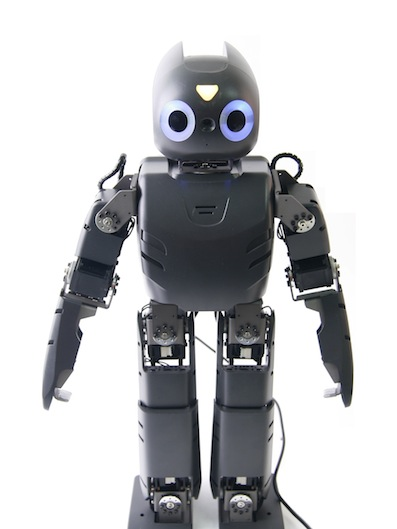
\includegraphics{darwin.png}}
%\caption{The DARWIN-OP Robot.}
%\label{fig:darwin}
%\end{center}
%\end{figure}

The NUbots team's major research focus is on using machine learning methods within the software systems of the robot to achieve increased performance and autonomy~\cite{ChalupEtAlSMC2007}. The current NUbots software source is available from \cite{nubotsGit} and is covered under the GPL. This includes associated toolkits for optimisation and learning on the robots. Our software platform is designed to work on multiple robotic platforms, and all of the individual modules have been designed with this in mind. The sensors and actuators are accessed using a standard format, regardless of the robot running the software~\cite{Kulk2011c}. 

The software is broken into a number of modules. The primary modules are: vision, localisation, behaviour, and motion. An overview of our software structure can be seen in Figure~\ref{fig:platform}. The research areas applied to each of these modules are described in the research section.

\begin{figure}[bht!]
\begin{center}
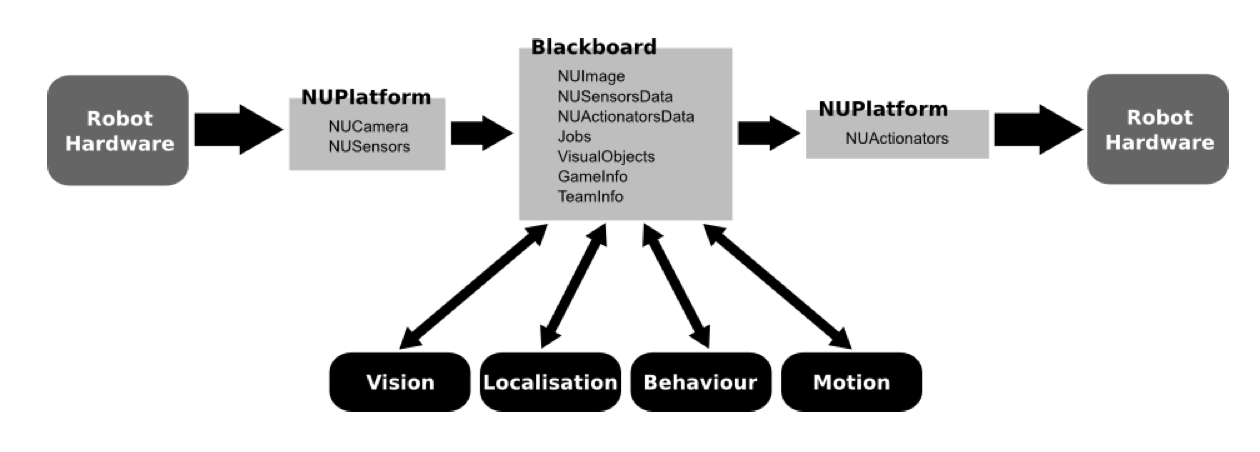
\includegraphics[width=1.0\textwidth]{Platform.png}
\caption{An overview of the software framework, and the transfer of information between the hardware and software modules via the blackboard~\cite{Kulk2011c}.}
\label{fig:platform}
\end{center}
\end{figure}


\section{Acknowledgement of Use of Code}
The NUbots Darwin-OP robots use a walk engine ported from the B-Human NAO robot walk engine \cite{BHumanWalk2010}. We acknowledge the source of this code and have made changes only in the areas that allow it to inter-operate with our multi-platform framework.

\section{Enhancements since RoboCup 2013}
Since Robocup 2013, improvements have been made in the area of software architecture and hardware. 

In response to the increase in field size, the Logitech C905 is being replaced with a Logitech C920. The new camera will provide a HD 1080p image, allowing the robots to detect and classify objects at a greater distance.

The Main Controller (CompuLab fit-PC2i) is being replaced by an ODROID-XU to help provide the extra processing power that is required for processing the HD images from the Logitech C920 while also allowing the software architecture to be further paralleled.

A prototype hardware replacement for the ROBOTIS CM730 Sub Controller, named the TAJ3850, is 
being developed as part of a Computer Engineering Third Year Project. The TAJ3850 provides power to all system components, a battery monitoring system featuring a low-voltage alarm and an extremely low-voltage automatic cut-off, a six-axis motion processing unit, a temperature sensor, and five dedicated motor buses. The TAJ3850 also exposes peripheral connections from the ODROID-XU to the back panel of the robot (HDMI, USB3, LAN, Audio output), monitors the three back-panel control buttons, and controls the status LEDs on the back panel and in the head.

\begin{figure}
\begin{center}
\scalebox{0.3}{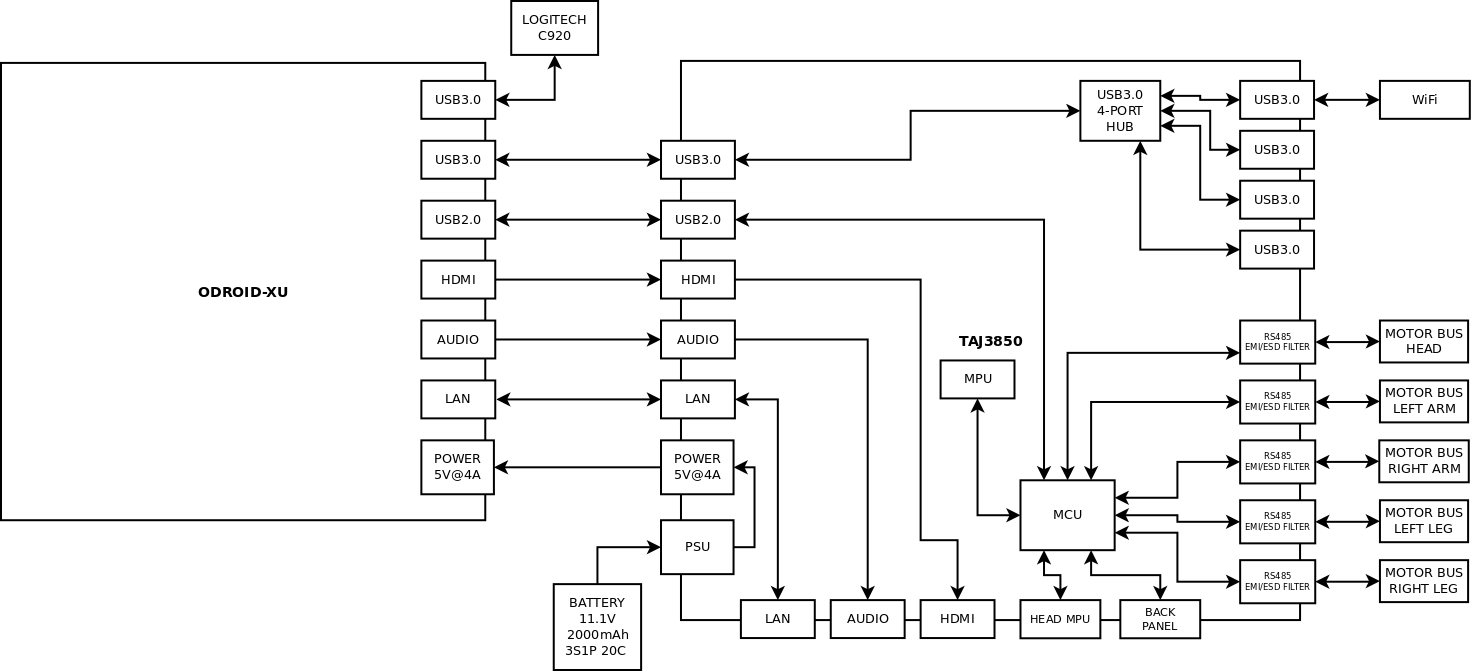
\includegraphics[angle=270]{TAJ3850.png}}
\caption{Connection mappings between the TAJ3850, ODROID-XU, and external peripherals.}
\label{fig:taj3850}
\end{center}
\end{figure}


The above enhancements will not be implemented on all of the Darwin-OP robots. The robots that do no get selected for these enhancement will have the standard Logitech C905, fit-PC21 and CM730 configuration.

\section{Research Areas}

\noindent\textbf{Robot Vision:} Vision is one of the major research areas associated with the Newcastle Robotics Lab. Several subtopics have been investigated including object recognition, horizon determination, edge detection, model fitting and colour classification using ellipse fitting, convex optimization and kernel machines. Recent work has resulted in a fully-autonomous method of colour look-up table generation using k-means clustering and support vector machines, as well as evaluation of colour spaces for unsupervised learning and occluded feature detection. Publications are available e.g. from~\cite{budden2012colour,budden2012ball,henderson_2007,nickin_2007,NUBOT2006,Henderson2008}.
\\

\noindent\textbf{Localisation and Kalman Filters:} Research on the
topic of localisation focused on Bayesian approaches to robot
localisation including Kalman Filter and particle filter
based methods. We are interested in 
modifications of the Kalman Filter to handle non-ideal information
from vision, incorporate increased information from multiple agents, 
and effectively utilise non-unique objects.
%Furthermore we are also interested in the use of machine learning to
%improve the models used by localisation. For information about our current approach see
%\cite{robocup_2009}.
\\

\noindent\textbf{Development of the Robot Bear:} In a collaborative
effort with the company Tribotix and colleagues in design a
bear-like robot (called Hykim) was developed~\cite{ChalupEtAl2006}. The idea was to have a modular open platform using high quality Dynamixel servos. 
\\

\noindent\textbf{Biped Robot Locomotion:} The improvement of walking speed and stability has been investigated by the NUbots since several years and on different platforms: On the AIBO robot we achieved one of the fastest walks at that time by walk parameter evolution \cite{QuinlanEtAlACRA2003,ChalupEtAlSMC2007}. On the Nao robot we improved existing walk engines by modifying the joint stiffnesses, or controller gains, \cite{Kulk2008,Kulk2010,Kulk2010a}. The stiffnesses were selected through an iterative process to maximise the cost of transport. We investigated the application of Support Vector Machines and Neural Networks to proprioception data for sensing perturbations during pseudo quiet stance. Walk improvements have been primarily done via optimisation techniques \cite{Kulk2011a,Kulk2011b} with recent improvements to our framework for online optimisation of bipedal humanoid locomotion. 
The use of spiking neural networks has been trialled in simulation~\cite{WiklendtChalup2008}. Prior to RoboCup 2012 the walk engine developed by the leading SPL team BHuman~\cite{BHumanWalk2010} was ported to the DARwIn-OP platform, and a variety of optimisation techniques were developed and successfully applied to improve walking speed and stability of the Darwin-OP. 
\\

\noindent\textbf{Reinforcement Learning, Affective Computing and Robot Emotions:} We investigate the feasibility of reinforcement learning or neurodynamic programming for applications such as motor control and music composition. Concepts for affective computing are developed in multidisciplinary projects in collaboration with the areas of architecture and cognitive science. The concept of emotion is important for selective memory formation and action weighting and continues to gain importance in the robotics community, including within robotic soccer. A number of projects in the Newcastle Robots lab already address this topic~\cite{ANFA2012,Pareidolia2010,HongEtAl2013a,HongEtAl2013b,WongEtAl2013}. 
\\

\noindent\textbf{Gaze analysis and head movement behavioural learning:} We investigated methods for human and robot pedestrian gaze analysis in~\cite{JalalianEtAl_CAADRIA2011,WongEtAl2012}. In another project we focus on detection analysis of salient regions/objects and wayfinding~\cite{BhatiaEtAl2012}. Recently we  applied reinforcement learning techniques to optimising head movement behaviour, providing a robust algorithm by which a robot learns to choose landmarks to localise efficiently during a soccer game. 
\\

\noindent\textbf{Manifold Learning:} In several projects we
investigate the application of non-linear dimensionality reduction
methods in order to achieve a better understanding and more precise
and efficient processing of high-dimensional visual and acoustic data.
\cite{ChalupEtAl2007b,WongChalup_WCCI_2008,WongChalup2008,WongEtAl2012}.
\\

\noindent\textbf{Other new projects:} Much work has been focused on the underlying software architecture and external utilities to enable flexibility and extensibility for future research. Projects undertaken include improving the configurability of the software system via parameter consolidation, development of a web-based online visualisation and debugging utility and the application of software architectural principles in the area of machine vision. Some of this work is currently still in progress as part of the 2012/2013 robotics lab summer projects by new undergraduate students who have joined the team.

\section{Related Research Concentrations}

The \emph{Interdisciplinary Machine Learning Research Group (IMLRG)} investigates different aspects of machine learning and data mining in theory, experiments and applications. Particular emphasis is put on interdisciplinary projects. The IMLRG's research areas include: Dimensionality reduction, vision processing, robotics control and learning, neurocomputing, evolutionary computation, optimisation, reinforcement learning, and kernel methods.

\noindent Links to publications can be found at the NUbots' webpage
\begin{center}
\texttt{http://robots.newcastle.edu.au/}
\end{center}

\bibliographystyle{plain}
% argument is your BibTeX string definitions and bibliography database(s)
\bibliography{nubots}

%%
%% ---- Bibliography ----
%%
%\begin{thebibliography}{12}
%\enlargethispage*{2mm}
%%\bibitem{robocup_2003} Jared Bunting, Stephan Chalup, Michaela
%%Freeston, Will McMahan, Rick Middleton, Craig Murch, Michael
%%Quinlan, Christopher Seysener, and Graham Shanks (2003).
%%\emph{Return of the NUbots! The 2003 NUbots Team
%%Report.}\\
%%\bibitem{TDP_2003} Stephan K. Chalup, Oliver J. Coleman, Michaela N. Freeston, Richard H. Middleton, Craig
%%L. Murch, Michael J. Quinlan, Christopher J. Seysener, and Graham D. Shanks (2003).
%%{\em The NUbots Team Description for 2003}. RoboCup 2003 Symposium.\\
%%\bibitem{robocup_2002} Chalup, S.,  Creek, N., Freeston, L., Lovell, N., Marshall, J., Middleton, R., Murch, C., Quinlan, M., Shanks, G.,
%%Stanton, C., and Williams, M.-A. (2002). \emph{When NUbots Attack~! The 2002 NUbots Team
%%Report.}
%%School of Electrical Engineering \& Computer Science Technical Report, The University of Newcastle, Australia.\\
%\bibitem{ChalupEtAl2006} S. K. Chalup, M. Dickinson, R. Fisher, R. H. Middleton, M. J.
%Quinlan, and P. Turner. {\em Proposal of a Kit-Style Robot as the
%New Standard Platform for the Four-Legged League}, In: Australasian
%Conference on Robotics and Automation (ACRA) 2006.\\
%
%\bibitem{ChalupEtAl2007} Stephan K. Chalup, Craig L. Murch, and Michael J. Quinlan. \emph{Machine Learning with AIBO Robots in the Four-Legged League of RoboCup}, IEEE Transactions on Systems, Man, and Cybernetics C, Vol. 37, No. 3, pages 297-310 May 2007.\\
%
%%\bibitem{ChalupMurchIFAC_2004} Stephan K. Chalup  and Craig L. Murch (2004). \emph{Machine Learning in the Four-Legged League}. 3rd IFAC Symposium on Mechatronic
%%Systems.\\
%
%\bibitem{ChalupHenderson2008} Chalup, S.K., Henderson, N., Ostwald, M.J. and Wiklendt, L. \emph{A Method for Cityscape Analysis by Determining the Fractal Dimension of Its Skyline}, ANZAScA 2008.\\
%
%\bibitem{ChalupHong2008} Chalup, S.K., Hong, K. and Ostwald, M.J. \emph{A Face-House Paradigm for Architectural Scene Analysis}, CSTST 2008 ACM 2008.\\
%
%\bibitem{ChalupEtAl2007b}  Stephan K. Chalup, Riley Clement, Joshua Marshall, Chris Tucker, and
%Michael J. Ostwald. \emph{Representations of Streetscape Perceptions
%Through Manifold Learning in the Space of Hough Arrays}.  2007 IEEE
%Symposium on Artificial Life, April 1-5, 2007. \\
%
%\bibitem{ChalupHenderson2009}
%Chalup, S.K., Henderson, N., Ostwald, M.J. and Wiklendt, L. \emph{A Computational Approach to Fractal Analysis of a Cityscape's Skyline}, Architectural Science Review, (forthcoming).\\
%
%%\bibitem{acal_2003} Oliver J. Coleman and Stephan K. Chalup (2003). \emph{Towards Matching Perception in Simulated and Real
%%World Robot Navigation}. Australian Conference on Artificial Life (ACAL'2003).\\
%%\bibitem{leonie_2002} Leonie Freeston (2002). \emph{Localization and World
%%Modelling,} project report, School of Electrical
%%Engineering and Computer Science, The University of Newcastle.\\
%
%%\bibitem{michaela_2003} Michaela Freeston (2003). \emph{Localisation and World Modelling in Robot Soccer}, project report, School of Electrical
%%Engineering and Computer Science, The University of Newcastle.\\
%\bibitem{henderson_2007} Henderson, N., King, R., and Middleton, R.H.
%(2007). \emph{An Application of Gaussian Mixtures: Colour Segmenting for the Four Legged League using HSI Colour Space}, RoboCup Symposium, Atlanta, July 2007. Lecture Notes in Computer Science , Springer-Verlag Berlin/Heidelberg, 2007.\\
%
%\bibitem{Henderson2008}
%Henderson, N., King, R., and Chalup, S.K. \emph{An Automated Colour Calibration System using Multivariate Gaussian Mixtures to Segment HSI Colour Space}, Proceedings of the 2008 Australasian Conference on Robotics \& Automation (ACRA'2008).\\
%
%%\bibitem{KohlStoneAAAI2004} Nate Kohl and Peter Stone (2004). Machine Learning for Fast Quadrupedal Locomotion. {\em The
%%Nineteenth National Conference on Artificial Intelligence}, AAAI 2004.\\
%
%\bibitem{Kulk2008} Kulk, J.A. and Welsh, J.S. \emph{A Low Power Walk for the NAO Robot}, Proceedings of the 2008 Australasian Conference on Robotics \& Automation (ACRA'2008).\\
%
%\bibitem{Kulk2010} Kulk, J.A. and Welsh, J.S. \emph{Autonomous Optimisation of Joint Stiffnesses over the Entire Gait Cycle for the NAO Robot}, Proceedings of the 2010 International Symposium on Robotics and Intelligent Sensors.\\
%
%%\bibitem{WilliamJarred_2002} McMahan, W. and Bunting, J. (2002). \emph{Vision
%%Processing}, project report, School of Electrical
%%Engineering and Computer Science, The University of Newcastle.\\
%
%%\bibitem{MurchChalup2004} Craig L. Murch and Stephan K. Chalup. \emph{Combining Edge Detection and
%%Colour Segmentation in the Four-Legged League}. Australasian
%%Conference on Robotics and Automation (ACRA'2004), 2004.\\
%
%%\bibitem{Murch2004} Craig L. Murch. \emph{Dimensionality Reduction on AIBO Robots}. Honours
%%Thesis, Newcastle Robotics Laboratory, 2004.\\
%
%\bibitem{nickin_2007} Nicklin, S.P, Fisher, R., and Middleton, R.H. \emph{Rolling shutter image compensation}.  Lecture Notes in Computer Science 4434, pages 402-409, Spinger-Verlag Berlin/Heidelberg, 2007.\\
%
%%\bibitem{traction2003} Quinlan, M., Murch, C., Middleton, R., and Chalup, S. (2003). \emph{Traction Monitoring for Collision Detection with Legged
%%Robots}. pp. 374 - 384, In: Daniel Polani, Brett Browning, Andrea Bonarini, and Kazuo Yoshida. RoboCup 2003: Robot Soccer World Cup VII, Lecture Notes in Computer Science 3020, Springer-Verlag 2004 (received engineering challenge paper award).\\
%%\bibitem{acra_2003} Quinlan, M.J., Chalup, S.K., and Middleton, R.H. (2003). \emph{Techniques for
%%Improving Vision and Locomotion on the Sony AIBO Robot}. Proceedings of the 2003 Australasian Conference on Robotics \& Automation (ACRA'2003).\\[-2mm]
%%\bibitem{nips_2003} Quinlan, M.J., Chalup, S.K., and Middleton, R.H. (2003). \emph{Application of SVMs for Colour
%%Classification and Collision Detection with AIBO Robots}. Advances
%%in Neural
%%Information Processing Systems (NIPS'2003).\\
%\bibitem{NUBOT2006} Quinlan, M.J., Nicklin, S.P., Henderson, N., Fisher, R., Knorn, F., Chalup, S.K., Middleton, R.H. and
%King, R. (2007) \emph{The 2006 NUbots Team Report.} School of
%Electrical Engineering \& Computer Science Technical Report, The
%University of
%Newcastle, Australia.\\
%%\bibitem{NUBOT2005} Quinlan, M.J., Nicklin, S.P., Hong, K., Henderson, N., Young, S.R., Moore, T.G., Fisher, R., Douangboupha, P., Chalup, S.K., Middleton, R.H. and King.
%%R. (2005). \emph{The 2005 NUbots Team Report.} School of Electrical
%%Engineering \& Computer Science Technical Report, The University of
%%Newcastle, Australia.\\
%%\bibitem{robocup_2004} Quinlan, M., Murch, C., Moore, T., Middelton, R., Lee,
%%Li., King, R, Chalup, S. (2004).  \emph{The 2004 NUbots Team
%%Report.} School of Electrical Engineering \& Computer Science Technical Report, The University of Newcastle, Australia.\\
%
%%\bibitem{seysener_2003} Seysener, C. (2003). \emph{Vision Processing for RoboCup 2003/2004}, project report, School of Electrical
%%Engineering and Computer Science, The University of Newcastle, 2003.\\
%
%%\bibitem{seysener_2004} Seysener, C., Murch, C., Middleton, R. (2004). \emph{Extensions to Object Recognition in the Four-Legged League}. pp. 274, In: RoboCup 2004: Robot Soccer World Cup VIII, LNCS 3276, Springer-Verlag 2005.\\
%
%\bibitem{WicklendtEtAl2008} Wiklendt, L., Chalup, S.K. and Middleton, R.H.. \emph{A Small Spiking Neural Network with LQR Control Applied to the Acrobot}, Neural Computing and Applications 17, Springer London 2008.\\
%
%
%\bibitem{WiklendtChalup2008}
%Wiklendt, L., Chalup, S.K. and Seron, M.M. \emph{Simulated 3D Biped Walking with and Evolution-Strategy Tuned Spiking Neural Network}, Neural Network World 19, pp. 235--246, 2009.\\
%
%\bibitem{WongChalup2008}
%Wong, A. and Chalup, S.K. \emph{Towards Visualisation of
%Sound-scapes Through Dimensionality Reduction}, 2008 IEEE World
%Congress on Computational Intelligence (WCCI), Hong Kong, June 1-6,
%2008.\\
%
%\bibitem{ChalupOstwald2009}Chalup, S.K. and Ostwald, M. J. \emph{Anthropocentric Biocybernetic Computing for
%Analysing the Architectural Design of House Fa\c{c}ades and Cityscapes. }, Design Principles and Practices: An International Journal Vol. 3, No. 5, pp. 65--80, ISSN: 1833-1874, 2009.\\
%
%\bibitem{Wong2008}
%%Wong, A.S.W. and Chalup, S.K. \emph{Sound-scapes for Robot Localisation through Dimensionality Reduction},  Proceedings of the 2008 Australasian Conference on Robotics \& Automation (ACRA'2008).\\
%
%\bibitem{robocup_2009}
%Naomi Henderson and Steven P. Nicklin and Aaron Wong and Jason Kulk and Stephan K. Chalup and Robert King (2009)
%\emph{The 2009 Nubots Team Report.} School of Electrical Engineering \& Computer Science Technical Report, The University of Newcastle, Australia.\\
%
%\bibitem{Kulk2010a}
%Jason Kulk and James Welsh \emph{Perturbation Sensing using Proprioception for Humanoid Robots.} Proceedings of the IEEE Conference on Robotics and Automation, 2010.
%
%\end{thebibliography}
%\enlargethispage*{5mm}

\end{document}
